\documentclass[conference]{IEEEtran}
%\IEEEoverridecommandlockouts
% The preceding line is only needed to identify funding in the first footnote. If that is unneeded, please comment it out.
\usepackage{cite}
\usepackage{amsmath,amssymb,amsfonts}
\usepackage{algorithmic}
\usepackage{graphicx}
\usepackage{textcomp}
\usepackage{xcolor}
\usepackage{caption}
\usepackage{subcaption}
\usepackage{multirow}
\graphicspath{ {/home/belfner/Documents/Spatial_Temporal_Mining/Project/paper/images} }
\def\BibTeX{{\rm B\kern-.05em{\sc i\kern-.025em b}\kern-.08em
		T\kern-.1667em\lower.7ex\hbox{E}\kern-.125emX}}
\begin{document}
	
	\title{Graph Based Approach to Unsupervised Clustering of USA Land Cover}
	
	\author{\IEEEauthorblockN{Benjaimin Elfner}
		\IEEEauthorblockA{\textit{CEAS} \\
			\textit{University of Cincinnati}\\
			Cincinnati, USA \\
			elfnerbm@mail.uc.edu}
	}
	
	\maketitle
	
	\begin{abstract}
		We present a method to create a clustering of land cover using planar graphs. Doing so transforms the problem into a vertex clustering one. This new representation is created using adjacent segments of land cover classes. Network representation techniques are then used to create component vectors for each node of the graph. These node representations are then clustered using standard clustering algorithms such as k-means or hierarchical to create regions with similar land patterns.
	\end{abstract}
	
	\begin{IEEEkeywords}
		clustering, NLCD, land cover, pattern analysis, graph representation
	\end{IEEEkeywords}
	
	\section{Introduction}
	Land cover analysis is crucial to forming decisions for tasks such as climate change or land management\cite{doi:10.1080/13658816.2015.1134796}. Regions can be formed by finding areas of land that exhibit similar spatial patterns of land cover also known as land pattern types (LPTs). These regions are important to many fields since they allow generalizations to be made of the land contained which can speed up analysis\cite{doi:10.1080/13658816.2015.1134796}. For example, measurements in one part of a region could apply to all related areas of land which reduces the work required to collect data.
	
	\section{Underling Data Mining Problem}
	For a given area of classified land cover (represented as a image), form regions of similar land pattern types. The regions formed should contain only sections of land that are similar with respect to the arrangement of the patches they are formed from. The regions should be useful meaning information is gained by combining the patches in the found arrangement.
	
	\section{Data Used}
	The data that will be used is the NLCD 2019 Land Cover (CONUS) dataset. This data, collected in
	2019, consists of a classification for each 30x30 meter square in the contiguous 48 US states.
	20 land cover classes describe the contents of the land cover for each square and are grouped into 8 superclasses. \cite{NLCD2019LandCover}
	
	\section{Related Works}
	Previously this problem was approached using the formation of motifels, small tiling subsections of the land cover data \cite{doi:10.1080/13658816.2015.1134796}. A co-occurrence histogram was created for each motifel where pixel adjacency are categorized and counted. These histograms can be compared to calculate a distance score for two motifels. Through a greedy algorithm, segments of contiguous motifel are grown until all surrounding motifels are no longer within a threshold distance of the motifel. Those segments are then clustered using hierarchical clustering. The benefit of this approach is reduced computational complexity since the data can be split into sections larger than a single pixel. The downside to this approach is the measure of similarity only considers the connections between two pixels and ignores larger patterns found in the data.
	
	
	\section{Our Approach}
	We will approach this problem by viewing land cover data as a planar graph. Each contiguous segment of land cover that shares a common class will represent the vertices and the edges are between adjacent segments. A possible modification of this method is to give a weight to each edge corresponding to the length of the shared perimeter. An example of this operation is shown in Fig. \ref{BasicTransform}. There are options to consider when creating graphs such as whether the graph should be weighted or unweighted as well as what if any prepossessing should be performed on the data.
	
	\begin{figure}[t]
		\centering
		\begin{subfigure}[b]{.4\textwidth}
			\centering
			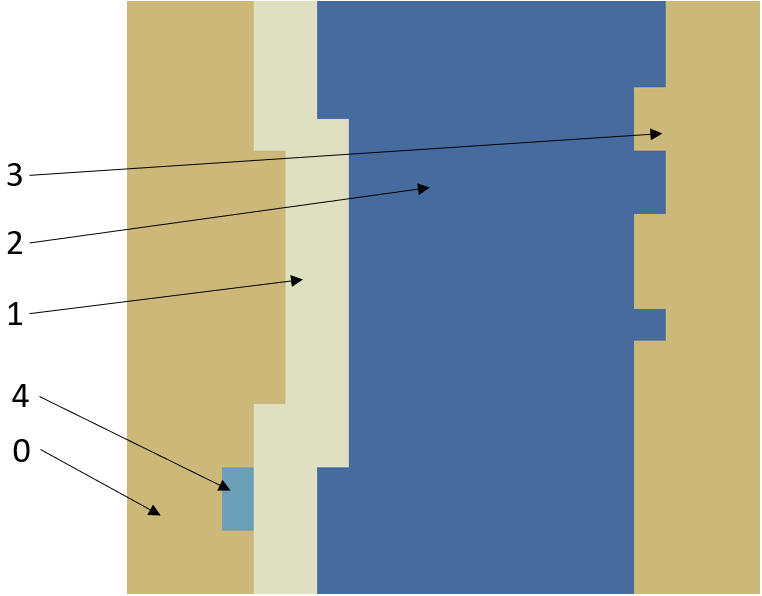
\includegraphics[width=\textwidth]{basic_landcover}
			\caption{Sample land cover}
			\label{Sample land cover}
		\end{subfigure}
		\vfill
		\begin{subfigure}[b]{.4\textwidth}
			\centering
			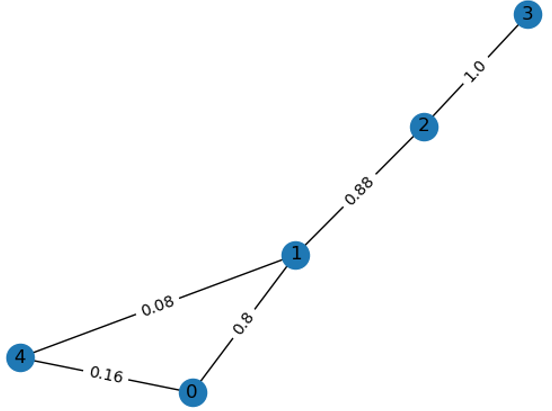
\includegraphics[width=\textwidth]{basic_landcover_graph}
			\caption{Resulting Graph}
			\label{Resulting Graph}
		\end{subfigure}
		\caption{This figure demonstrates how a section of land cover is converted into a graph. Each of the labeled sections of the image correspond to the node with the same label. The weights on the graph are the length of the shared perimeter relative to the length of the largest perimeter observed in the image which in this case is the one between 2 and 3.}
		\label{BasicTransform}
	\end{figure}
	
	With this representation, new approaches can be used to compare vertices of the graph. In this paper, we will be comparing three methods. These methods were selected due to their varying methodologies, optimization methods, and experimental performance. Basic details are given in TABLE \ref{NWRC}.
	
	Each method produces vector embedding for each vertex of the graph. These vectors will be clustered using a classic partitioning clustering method.
	
	\renewcommand{\arraystretch}{1.2}
	\begin{table*}[t]
		\begin{tabular}{|l|l|l|l|}
			\hline
			Method & Complexity      & Structure Captured     & Training Method                              \\
			\hline
			LINE   & $O(d|E|)$         & \multirow{2}{*}{Local} & \multirow{2}{*}{Stochastic Gradient Descent} \\
			\cline{1-2}
			LGAE   & $O(d|V|)$         &                        &                                              \\
			\hline
			GraRep & $O(|V||E|+d|V|2)$ & Global                 & Eigen Decomposition \\
			\hline
		\end{tabular}
		\caption{Comparison of basic attributes of the selected network representation methods \cite{zhang2018network}\cite{SalhaGalvan2019KeepIS}}
		\label{NWRC}
	\end{table*}
	\renewcommand{\arraystretch}{1}
	
	\subsection{LINE \cite{Tang2015LINELI}}
	LINE creates vector representations for each vertex and can create these embedding to represent either the first or second-order proximity. 
	
	\subsection{Linear Graph Autoencoders \cite{SalhaGalvan2019KeepIS}}
	An autoencoder is a model that is able to take data and convert it to a different representation of the data. Most of the time this new representation has reduced dimensionality or can represent the original data in a new format that is more conducive to other data mining tasks. The strength of an autoencoder is judged on its ability to recreate the input from the reduced form. A graph autoencoder is able to convert a vertex to a vector representation.
	
	\subsection{GraRep \cite{Cao2015GraRepLG}}
	GraRep creates a vector of step representations for each vertex on a graph. The ${k}$th value in the vector encodes information about graph ${k}$ steps from the vertex.
	
	\section{Understanding Limitations of Approach}
	Clustering land cover patches has several inherit issues. First, the algorithms used to cluster the nodes are unaware of the class labels for each. This means when comparing the two nodes, the only information available is the nodes connections to other nodes. This leads to issues where two patches of the same class that could be considered part of the same pattern if their class is taken into account but because the structure of the surrounding nodes is not quite similar enough for the algorithms to come to the same conclusion.
	
	
	Another issue is the variance in the sizes of patches. As seen in Figure \ref{size_distribution_example}, the range of patch sizes is very large and the distribution is heavily skewed towards the smaller patches. The size calculations do not take into account any portion of the patches that are clipped by the image so the actual max patch size is larger than stated. Having a disproportionate mix of very large and very small areas causes issues for both.
	
	Large areas cause distant areas to be only a few steps away. This causes any algorithm analyzing the structure of the graph to assume that all areas connected to a large area to be closely related to each other. Another issue is the algorithms are only able to assign each patch to 1 region. For small regions this is not a problem since the difference of placing a border patch in one region or another has little effect on the overall structure of the regions, but for large regions it is unreasonable to assume they fit that neatly into the categories due to there size (EVIDENCE NEEDED).
	
	Small patches have the opposite issue to the first of the large patches. Small patches could be spatially close to each other but if they are in a dense region of many small patches the path between the two patches on the graph could be many steps. This disparity between the large and small regions makes it difficult to come up with a simple solution that addresses both issues.
	
	\begin{figure*}[t!]
		\centering
		\begin{subfigure}[b]{0.4\textwidth}
			\centering
			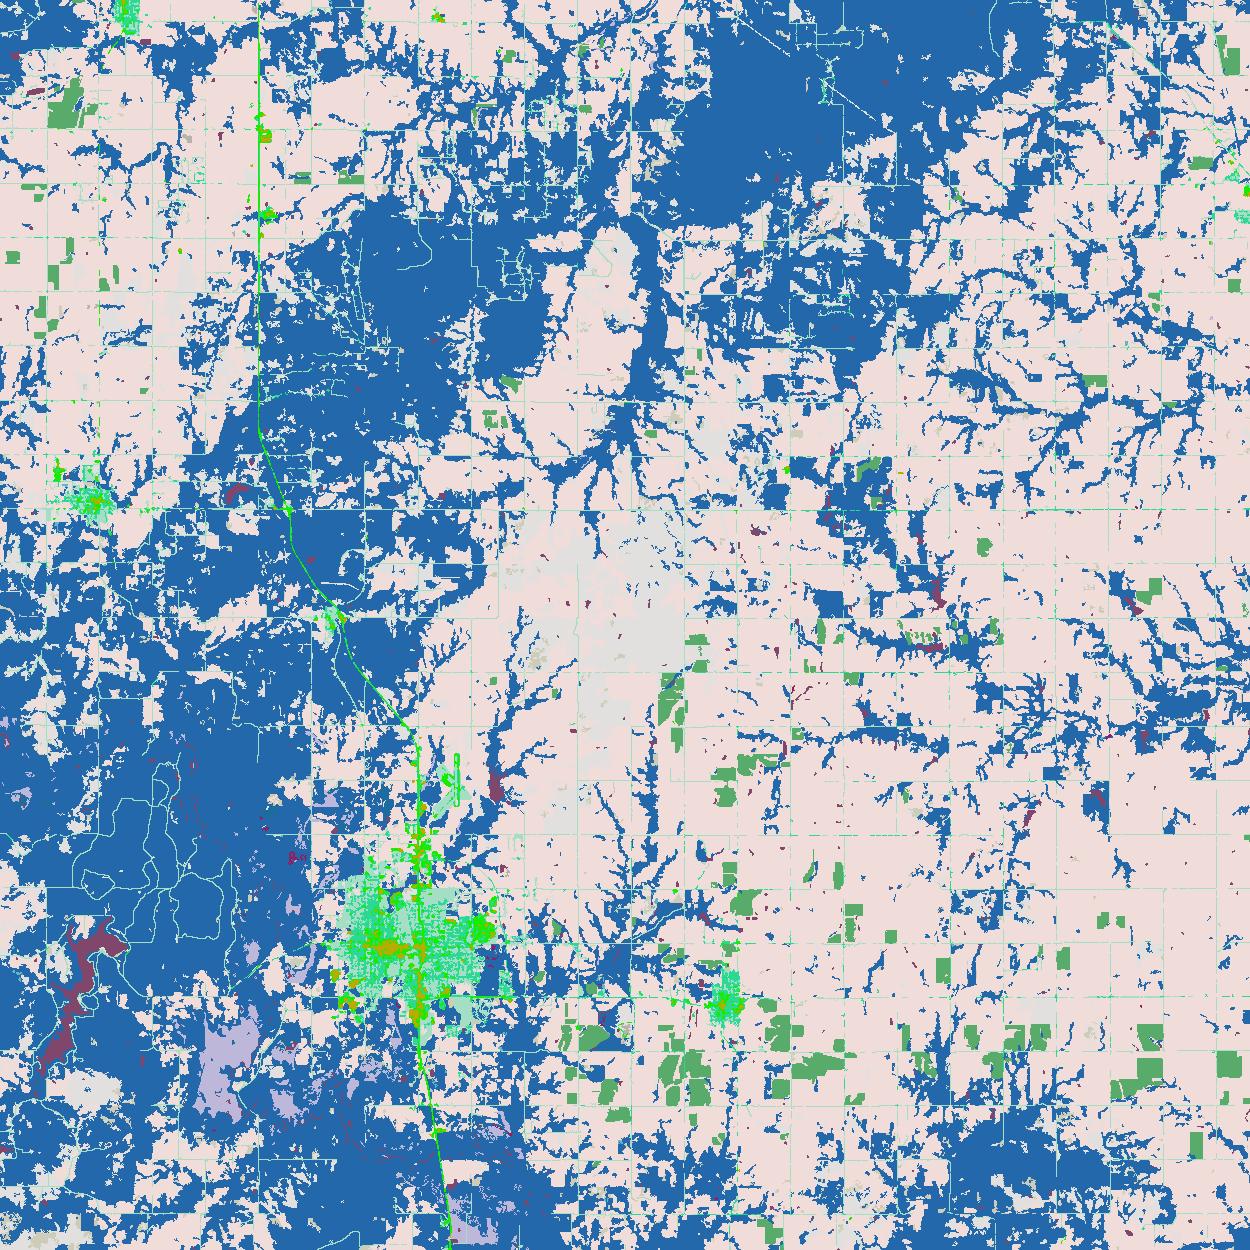
\includegraphics[width=\textwidth]{size_dist_landcover}
			\caption{Sample Land Cover}
			\label{simple_land_cover}
		\end{subfigure}
		\hfill
		\begin{subfigure}[b]{0.45\textwidth}
			\centering
			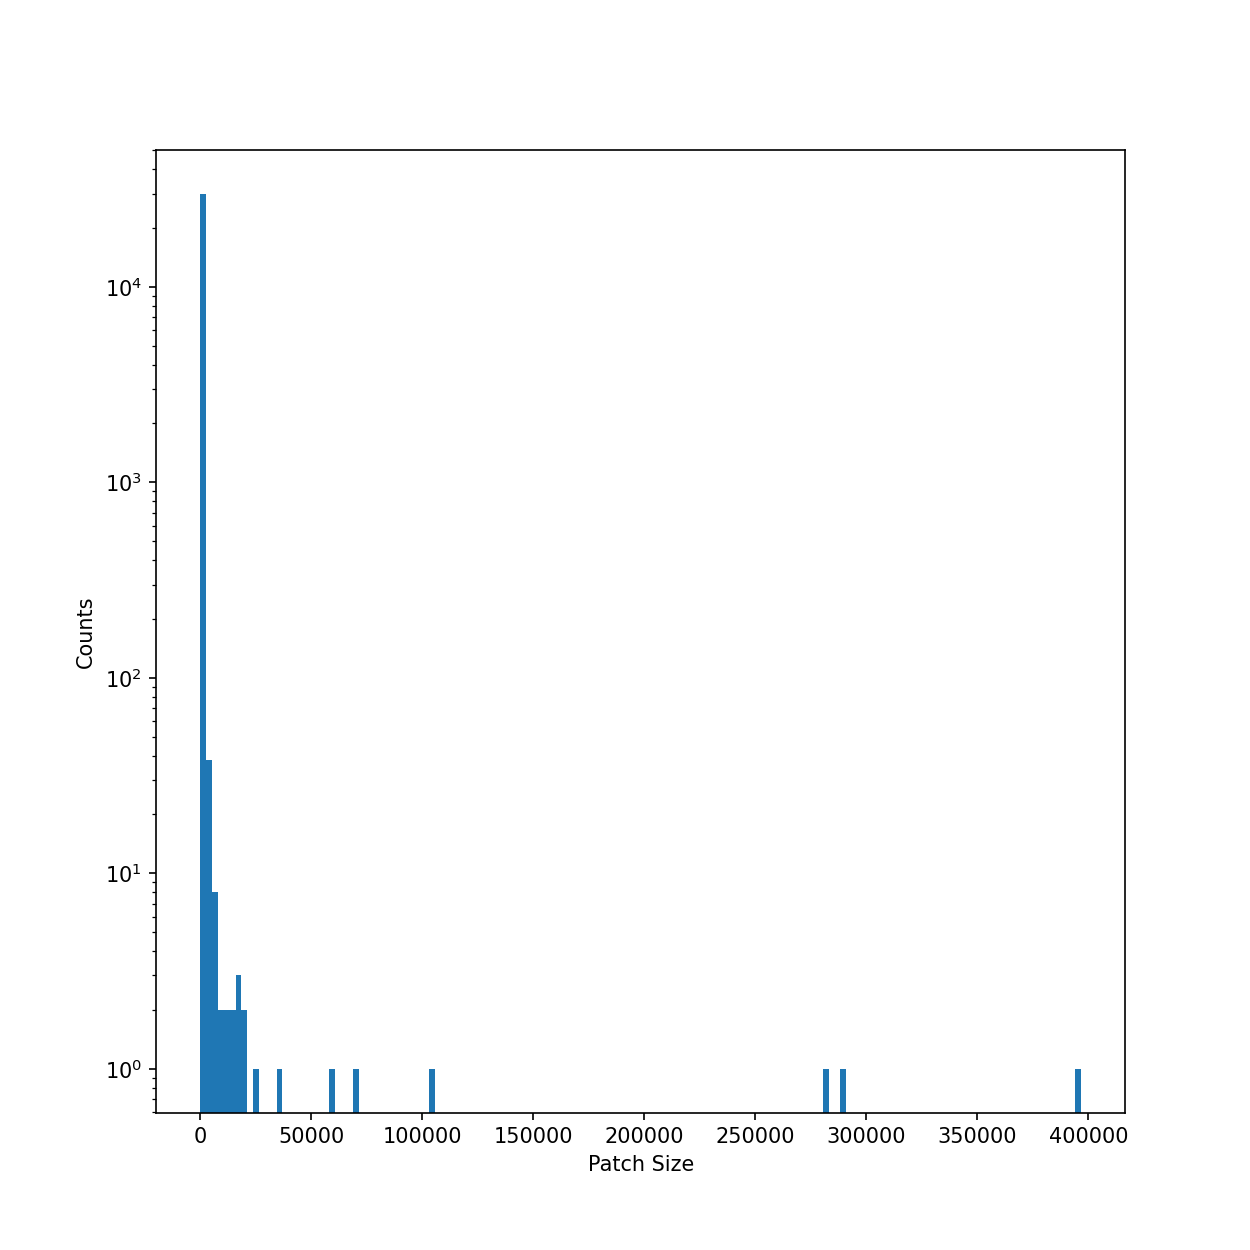
\includegraphics[width=\textwidth]{size_dist}
			\caption{Size Distribution}
			\label{size_distribution}
		\end{subfigure}
		\begin{subfigure}[b]{0.45\textwidth}
			\centering
			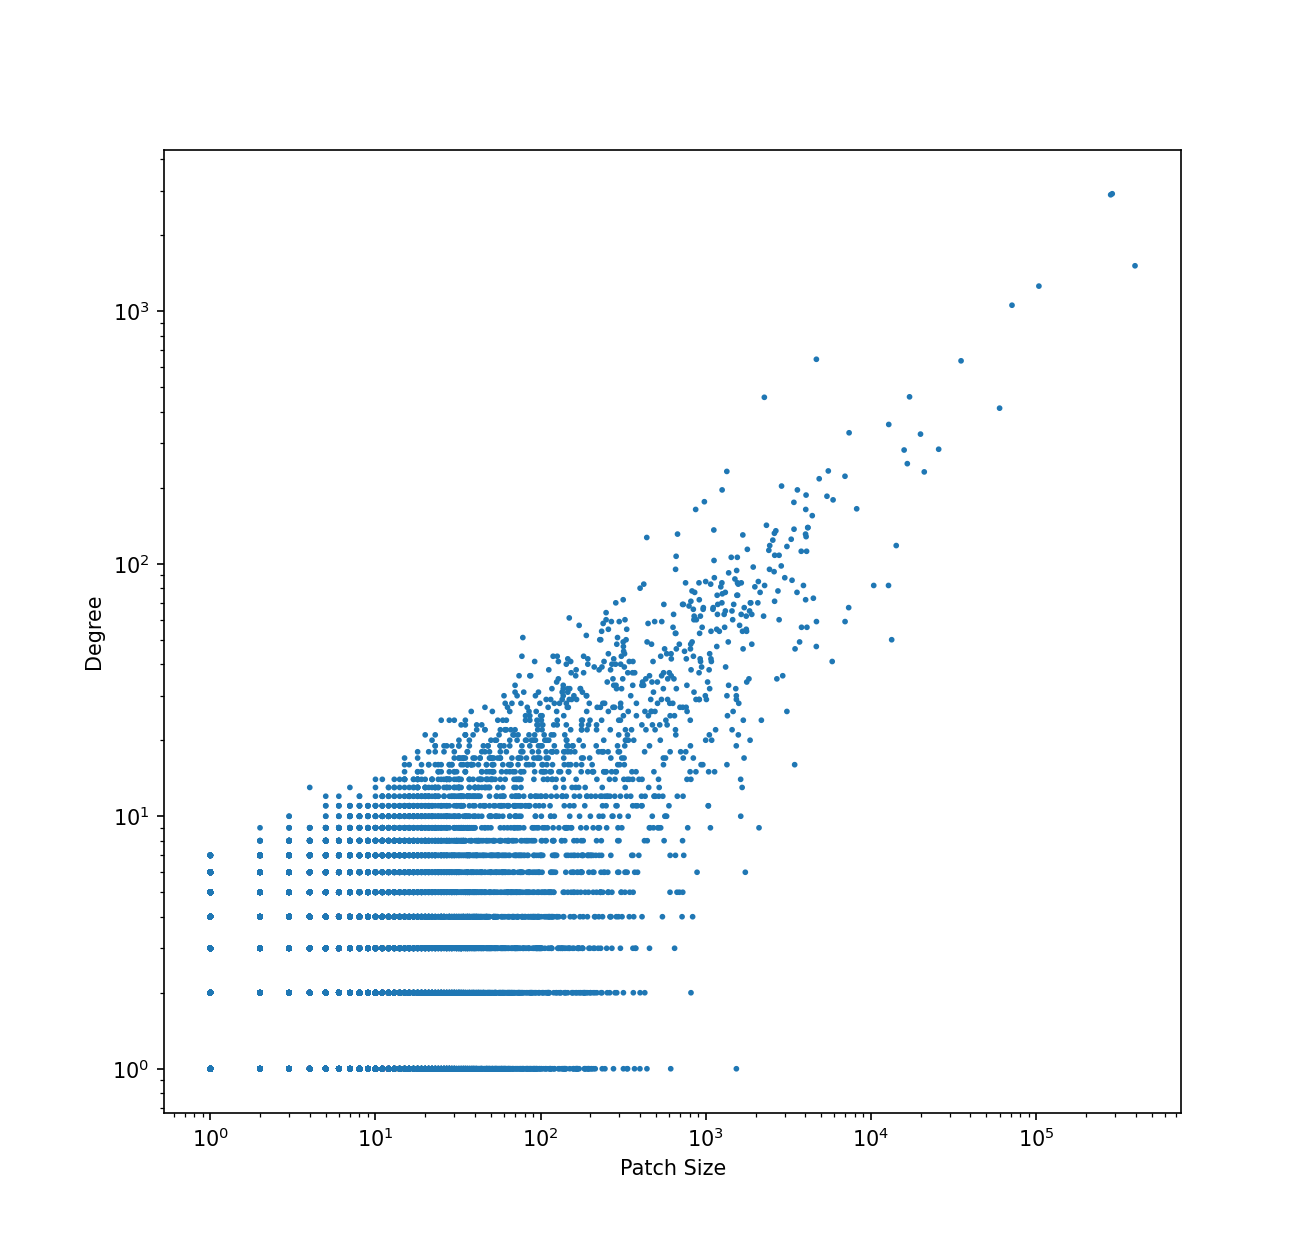
\includegraphics[width=\textwidth]{degree_dist}
			\caption{Degree vs Area}
			\label{degree_vs_area}
		\end{subfigure}
		\caption{This figure shows the distribution of patch sizes as well as the relationship between area and degree of the patches from a random section of landcover. In \ref{size_distribution} this example 80\% of the patches have an area of 9 pixels or less while the range of sizes is 1 to 52686 pixels.}
		\label{size_distribution_example}
	\end{figure*}
	
	\subsection{Posible Solutions}
	There are several possible solutions to these issues but they all have strengths and weaknesses. 
	
	\begin{itemize}
		\item Lack of Node Label Information
		\begin{itemize}
			\item Append one-hot encoding data to component data found by algorithms. This provides the node label information to the clustering algorithms but it can also encourage the algorithm to wrongly assume distant patches are more related only because they are of the same class. There are also the issue of how to weight the class data compared to the component data found by the graph encoding algorithms.
		\end{itemize}		
		
		
		\item Large Patches
		\begin{itemize}
			\item Split large regions into smaller areas. This prevent spatially distant patches from being only a few hops away and allows them to be part of different regions but how they should be split is ambiguous and can introduce artifacts into the data (EVIDENCE NEEDED). Things to consider when splitting patches is the shape and size of the formed subpatches as well as there distribution.
			\item Drop large regions. This prevents the shortest path between spatially distant patches from traversing through the large patches but this can can introduce artifacts into the data (EVIDENCE NEEDED) as well as creating disjoint graphs.
		\end{itemize}
		\item Small Patches
		\begin{itemize}
			\item Merge smaller patches into larger groups. This reduces the spatial density of areas with many small patches allowing the new patches to be closer to surrounding patches on the graph but information is destroyed in the process. Also selecting which patches to be merged, how patches should be merged, and what their new class label should be has many different approaches each with there own consequences (EVIDENCE NEEDED). Some examples of merging rules is all patches with an area less than 4 pixels are merged into the neighbor they share the most perimeter with and the new patch retains the class label of the larger region. 
			\item Simplify patch labels to only reference super categories. Provided with the land cover data is a categorization of the present classes. The land cover patches present in a landcover sample can be reduced to their supercategory and merged with neighboring patches of the same supercategory. This reduces the number of small patches as some will be nearby patches of the same supercategory but this has consequences such as with roads which by their connected nature usually merge with all other road patches on the sample which can connect very distant patches to each other (EVIDENCE NEEDED).
		\end{itemize}
	\end{itemize}	
	
	\section{Proposed Research}
	\subsection{Plan}
	\begin{itemize}
		\item Finish implementation of Linear Graph Autoencoders - 5 April 2022
		\begin{itemize}
			\item Understand the parts of the algorithm mathematically
			\item Create toy model to understand it in a more overall sense
		\end{itemize}
		
		\item Finish implementation of LINE - 10 April 2022
		\begin{itemize}
			\item Understand the parts of the algorithm mathematically
			\item Create toy model to understand it in a more overall sense
		\end{itemize}
		
		\item Begin running tests on the entire pipeline - 15 April 2022
		\item Have all changes finalized - 20 April 2022
	\end{itemize}
	
	
	\section{Evaluation}
	The resulting trees for each embedding algorithm can be split such that a desired number of regions are formed. Due to this fact as well as the methods being unsupervised means the resulting regions do not have any human-defined meaning nor can the clusters be quantitative compared a ground truth. Therefore, the assessment will be based solely on the usefulness of the clusters. This will be done by examining the patterns found in each cluster qualitatively. The resulting clusters structure will also be compared to regions created by human conducted surveys.
	
	\subsection {Results}
	Example Result of Pipeline
	\begin{itemize}
		\item Input image: 30x30 km region near New Orleans, LA
		\item Number of segments: 8096
		\item Network Representation Method used: GraRep
		\item GraRep Arguments:
		\begin{itemize}
			\item k=5
			\item d=5
		\end{itemize}
		\item Clustering Method: Hierarchical with ward linkage
		
	\end{itemize}
	Results can be viewed in Fig. \ref{Pipeline results}
	\begin{figure*}[t!]
		\centering
		\begin{subfigure}[b]{0.4\textwidth}
			\centering
			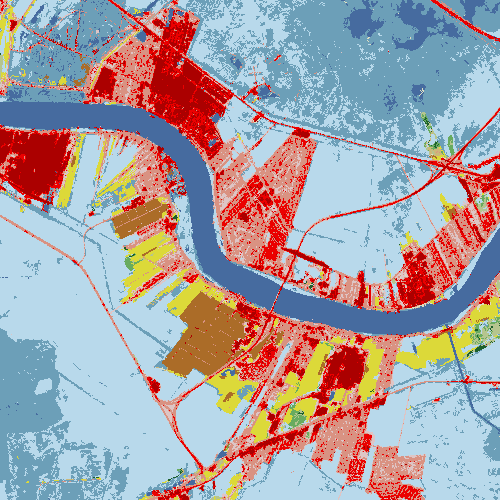
\includegraphics[width=\textwidth]{landcover}
			\caption{Land cover classes}
			\label{base}
		\end{subfigure}
		\hfill
		\begin{subfigure}[b]{0.4\textwidth}
			\centering
			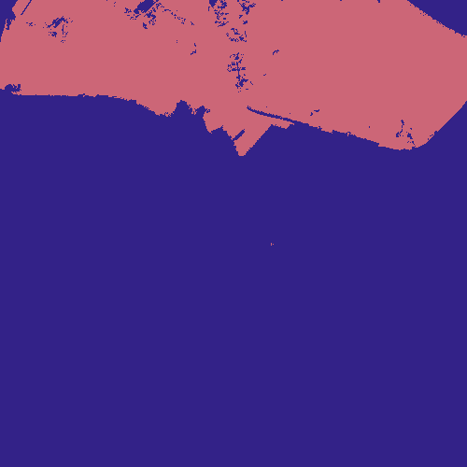
\includegraphics[width=\textwidth]{2clusters}
			\caption{2 clusters}
			\label{2 clusters}
		\end{subfigure}
		\hfill
		\begin{subfigure}[b]{0.4\textwidth}
			\centering
			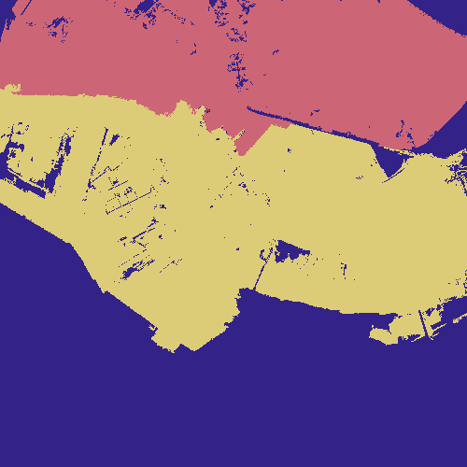
\includegraphics[width=\textwidth]{3clusters}
			\caption{3 clusters}
			\label{3 clusters}
		\end{subfigure}
		\hfill
		\begin{subfigure}[b]{0.4\textwidth}
			\centering
			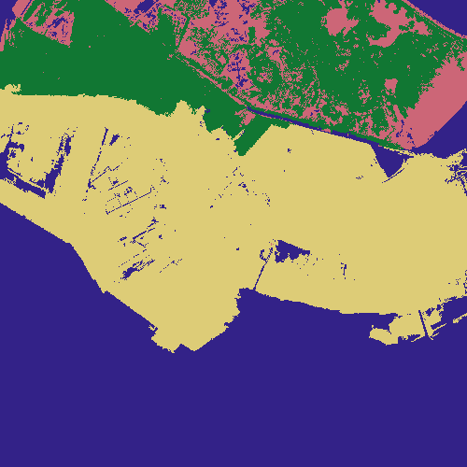
\includegraphics[width=\textwidth]{4clusters}
			\caption{4 clusters}
			\label{4 clusters}
		\end{subfigure}
		\caption{Pipeline results}
		\label{Pipeline results}
	\end{figure*}
	
	
	
	\section{Conclusion}
	This paper explores graph representations of land cover and has shown its merits as a technique to be used for clustering land cover based on the patterns found within it. It has also shown how re-representing the spatial data influences the resulting clusters and what modifications to the conversion process can be introduced to avoid shortcomings present in the new format. What has been discussed here is only intended as a preliminary exploration into the abilities and merits of graph-based land cover clustering and many more ideas from all fields can be applied to this problem in the future.
	
	
	
	\bibliographystyle{IEEEtran}
	\bibliography{./references}
	
	
\end{document}
